
\section{Modely}
\label{sec:modely}
Všetky modely pre trénovanie su implementované v scripte \textit{models.py}.
Existuje jedna hlavná trieda \textit{class Model}, ktorá obsahuje všetky základne atributy potrebné pre modely, ako npr.
    meno modelu, vstupný rozmer dát, zvolený algoritmus trénovania a štruktúru typu dictionary ktorá obsahuje indexi a názvi označení obrázkov.

Každý model následne dedí z tejto hlavnej triedy a implementuje v sebe 2 funkcie \textit{build} ktorá zabezpečuje vytvorenie modelu a
    funkciu \textit{train} ktorá sa volá pri spustení trénovania daného modelu.

\begin{figure}[H]
    \centering
    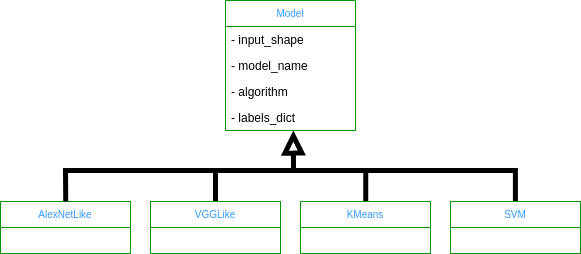
\includegraphics[width=0.8\textwidth]{inheritance}
    \caption{Hierarchia dedenia tried modelov.}
    \label{pic:inheritance}
\end{figure}

Konvolučné neurónové siete su implementované pomocou triedy \textit{Sequencia} z knižnice Keras.
Pre klasifikátor K-Nearest-Neighbor je použitá trieda \textit{KNeighborsClassifier} a trieda \textit{SVC} pre klasifikátor SVM z knižnice scikit-learn.
%Pre klasifikátor K-Nearest-Neighbor je použitá trieda \textit{KNeighborsClassifier} s počtom 1 a 5 najbližších susedov, a trieda \textit{SVC} pre klasifikátor SVM
%    so základnymi nastavenia trénovania z knižnice scikit-learn.

\subsection{Ukladanie a načitanie modelu}
\label{subsec:ukladaniemodelu}
Pre ukladanie natrénovaných modelov je implemtovaná funkcia \textit{save\_model()} v triede \textit{DataSaver} v scripte \textit{loader.py}.
Pri ukladaní modelu sa ukladá model v binárnej forme, ukladá sa konfiguračný súbor \textit{settings.json} ktorý obsahuje informácie ako veľkosť
    vstupných dát, použité funkcie na predspracovanie dát, meno modelu, typ algoritmu učenia, zoznam indexov označenia dát a dalšie informácie
    špecifické pre daný typ modelu.
Uložením konvolučnéj neurónovej siete sa ukladá graf priebehu trénovanie.

Naopak pre načitanie modelov je implementovaná funkcia \textit{load\_model\_data()} v triede \textit{DataLoader} v scripte \textit{loader.py},
    ktorá načíta binárnu podobu modelu a všetky informácie z konfiguračného súboru \textit{settings.json}.
